\chapter{In depth flight analysis}
\label{sec:specific_runs}

In the following, a detailed flight log is shown for the test setting of spawning at a fixed location on the Arroyo map and flying a random mission at 100 m altitude.

This example shows an ordinary flight where the drone took off from the ground, flew to a mission way point at cruise altitude and attempted to land twice which the second attempt was successful.

\section{Trajectory and landing position}

As for \cref{chapter:evaluation}, the landing attempts are shown in \cref{fig:demo_run_landing}.

\begin{figure}[h]
\centering
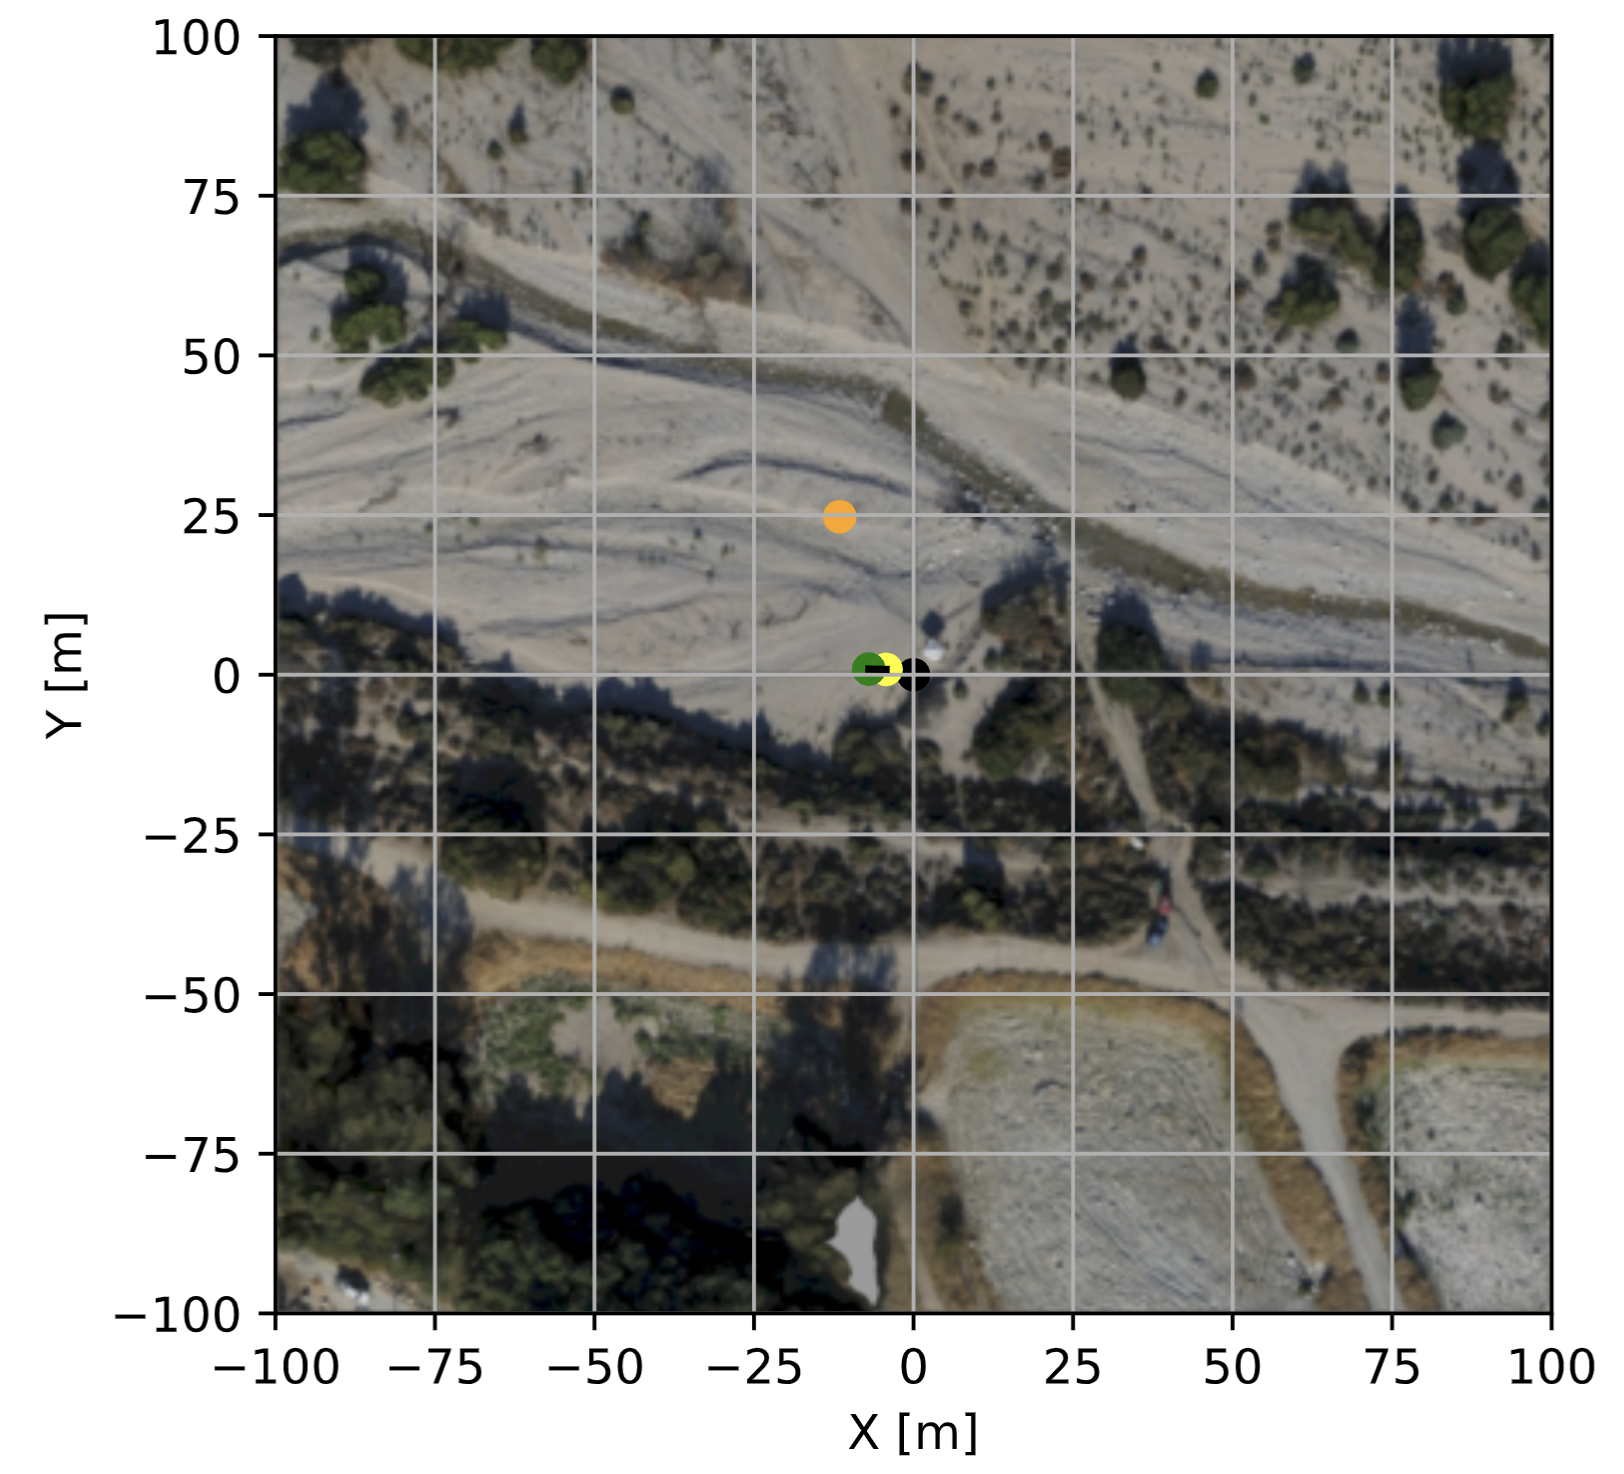
\includegraphics[scale=0.45]{images/appendix/run_analysis/demo_run.png}
\caption{Visual Analysis of demo landing: Black is the spawn of the drone, orange indicated the mission way point, yellow the first landing attempt which wasn't verified and green shows the final successful landing attempt.}
\label{fig:demo_run_landing}
\end{figure}

The mission way point in this run was quite close to the center. Therefore, it comes to no surprise that a landing site at the start plateau was chosen. One landing site was chosen but not verified and a close by site was subsequently chosen.

To show the path taken by the drone \cref{fig:lateral_trajectory} shows the x-y plot of the flight.

\section{Autonomy Log}

A summarizing log containing the most important information is shown below:

\begin{lstlisting}
    -----------------
    Iteration1:
    Spawn Randomization Disabled - Drone spawns at arroyo's \n
    
    default position: 0 0 0 0 0 3.5
    No additional landing sites spawned.
    Mission Waypoints added:
    Waypoint 0: (x: -24.739966478190148, y: -11.563968813290693, z: 100.0)
    --------
    Evaluation 1
    --------
    Run took 384.94275641441345s
    Landing Site Log:
    LS 1: [2024-04-21_23:44:43] [INFO]  Selecting Landing Site \n
    
    with ID 12 at (x: -0.834371, y: -4.30025, z: -0.4452)

    Landing Site Verification 1: Failure
    LS 2: [2024-04-21_23:47:26] [INFO]  Selecting Landing Site \n
    
    with ID 1834 at (x: -0.884371, y: -7.00025, z: -0.533367)

    Landing Site Verification 2: Successful
    Landing Sequence was initiated
    Checks:
    Rotation Check: Successful

    Conclusion: Success
    ---------------------------------
\end{lstlisting}

The log shows the spawn position at the usual location introduced in \cref{fig:fixed_start} in the evaluation. 


